\documentclass{beamer}
\usetheme{Madrid}
\usecolortheme{whale}
\usepackage{tikz}
\usetikzlibrary{automata, positioning, arrows.meta}
\usepackage[utf8]{inputenc}
\usepackage[T1]{fontenc}
\usepackage[french]{babel}
\usepackage{amsmath, amssymb}

\title[Automate de l'électeur]{Automate cellulaire probabiliste de l'électeur}
\subtitle{Analyse markovienne et simulations numériques}
\author[Groupe 48]{Django CHEVALLET \and Paul-Aliocha CORDONNIER \and Augustin MANIAK \and Racim ZENATI}
\institute[]{ENSIMAG}
\date{18 décembre 2025}

\begin{document}

\begin{frame}
  \titlepage
\end{frame}

\section{Introduction et Modèle}

\begin{frame}{Le Modèle de l'Électeur (Holley \& Liggett, 1975)}
  \begin{itemize}
    \item \textbf{Définition} : Processus aléatoire en temps discret sur une grille $M$ de dimension $d$[cite: 287, 288].
    \item \textbf{État d'une cellule} : $\xi_n(x) \in \{0, 1\}$ (modèle simple)[cite: 293].
    \item \textbf{Règle d'évolution} : Une cellule adopte la valeur d'un de ses voisins choisi uniformément[cite: 295].
    \item \textbf{Probabilité de transition} :
    \[ p_{x}(i) = \frac{\text{card}\{y \in \mathcal{N}_x, \xi_n(y) = i\}}{\text{card} \mathcal{N}_x} \]
  \end{itemize}
  \end{frame}

\begin{frame}{Cadre Théorique : Chaînes de Markov}
  \begin{itemize}
    \item \textbf{Processus de Markov} : L'évolution future ne dépend que de l'état présent[cite: 289, 297].
    \item \textbf{Matrice de Transition $P$} : $P_{i,j} = \mathbb{P}(\xi_{n+1} = j \mid \xi_n = i)$[cite: 300, 302].
    \item \textbf{Propriétés clés} :
    \begin{itemize}
        \item Homogénéité temporelle[cite: 310].
        \item Espaces d'états finis : $|\mathcal{S}| = \kappa^{N^d}$[cite: 304, 510].
        \item Classification des états : Récurrents vs Transitoires[cite: 323, 324].
    \end{itemize}
  \end{itemize}
\end{frame}

\section{Dimension 1 : Analyse Spectrale et Convergence}

%2 Django
\begin{frame}{Puissances de la matrice de transition}
\begin{itemize}
  \item Soit $(X_n)_{n \geq 0}$ une chaîne de Markov de matrice de transition $P$.
  \item Pour tout $n \geq 0$ et pour tous états $i,j \in \mathcal{S}$ :
  \[
  (P^n)_{ij} = \mathbb{P}(X_n = j \mid X_0 = i)
  \]
  \item La matrice $P^n$ donne donc directement les probabilités de transition en $n$ pas.
\end{itemize}
\end{frame}

%2.1 Django
\begin{frame}{Cas de N = 2 à bords opposés}
\begin{itemize}
  \item Pour une chaîne de Markov :
  \begin{itemize}
    \item finie,
    \item irréductible,
    \item positivement récurrente.
  \end{itemize}
  \item Il existe une unique mesure stationnaire $\pi$.
  \item Pour tout état $i \in \mathcal{S}$, on a la relation fondamentale :
  \[
  \pi_i = \frac{1}{\mathbb{E}[T_i^+]}
  \]
  où $T_i^+$ est le temps de retour en $i$ :
  \[
  T_i^+ = \inf\{ n \geq 1 \mid X_n = i \mid X_0 = i \}
  \]
\end{itemize}
\end{frame}

%2.1 Django
\begin{frame}{Cas $N=2$ à bords opposés : chaîne associée}
\begin{itemize}
  \item La chaîne de Markov associée à N = 2 à bords opposés admet la matrice de transition :
  \[
  P =
  \begin{pmatrix}
  \tfrac12 & \tfrac12 & 0 & 0 \\
  \tfrac14 & \tfrac14 & \tfrac14 & \tfrac14 \\
  \tfrac12 & \tfrac12 & 0 & 0 \\
  0 & \tfrac12 & 0 & \tfrac12
  \end{pmatrix}
  \]
  \item Chaque état communique avec tous les autres : la chaîne est donc irréductible.
  \item L’espace d’états étant fini, tous les états sont récurrents positifs.
  \item La chaîne admet donc une loi stationnaire unique.
\end{itemize}
\end{frame}

%2.1 Django
\begin{frame}{Calcul de la loi stationnaire}
\begin{itemize}
  \item La mesure stationnaire $\pi = (\pi_0,\pi_1,\pi_2,\pi_3)$ vérifie :
  \[
  \pi = \pi P
  \]
  \item Cela conduit à un système linéaire issu des équations de balance :
  \[
  \begin{cases}
  \pi_0 = \tfrac12 \pi_0 + \tfrac14 \pi_1 + \tfrac12 \pi_2 \\
  \pi_1 = \tfrac12 \pi_0 + \tfrac14 \pi_1 + \tfrac12 \pi_2 + \tfrac12 \pi_3 \\
  \pi_2 = \tfrac14 \pi_1 \\
  \pi_3 = \tfrac12 \pi_3 + \tfrac14 \pi_1
  \end{cases}
  \quad \text{avec } \sum_i \pi_i = 1
  \]
  \item La résolution donne :
  \[
  \pi = [0.3 \; ; \; 0.4 \; ; \; 0.1 \; ; \; 0.2]
  \]
  \item En utilisant le lien entre probabilité stationnaire et temps de retour on a estimé empiriquement les temps de retour moyen (1 milion d'itérations) on obtient :
  \[
  \pi' = [0.22 \; ; \; 0.44 \; ; \; 0.11 \; ; \; 0.22]
  \]
\end{itemize}
\end{frame}

\begin{frame}{Cas $N=2$ à bords égaux}
  \begin{columns}
    \begin{column}{\textwidth}
      \begin{itemize}
        \item \textbf{Configurations} : 1001 (A), 1011 (B), 1101 (C), 1111 (D).

\begin{figure}[H]
  \begin{center}
    \begin{tikzpicture}[-latex, auto, node distance = 4cm, on grid,
        state/.style = { circle, draw }
      ]
      \node[state] (A) {A};
      \node[state] (B) [above right = of A] {B};
      \node[state] (C) [below right = of B] {C};
      \node[state] (D) [below left = of C] {D};

      \path (A) edge [loop left] node[left] {$1/4$} (A);
      \path (A) edge [bend left] node[left] {$1/4$} (B);
      \path (A) edge [bend right] node[left] {$1/4$} (C);
      \path (A) edge [bend right] node[left] {$1/4$} (D);
      \path (B) edge [bend left] node[left] {$1/2$} (C);
      \path (B) edge [bend right] node[left] {$1/2$} (D);
      \path (C) edge [bend left] node[left] {$1/2$} (B);
      \path (C) edge [bend left] node[left] {$1/2$} (D);
      \path (D) edge [loop below] node[left] {$1$} (D);
    \end{tikzpicture}
  \end{center}
  \caption{Automate probabiliste pour $N = 2$ à bords égaux}
\end{figure}

      \end{itemize}
    \end{column}
  \end{columns}
\end{frame}

\begin{frame}{Cas $N=2$ à bords égaux}
  \begin{columns}
    \begin{column}{\textwidth}
      \begin{itemize}
        \item \textbf{matrice de transition agrégée} : 
\[
P =
\begin{pmatrix}
\frac14 & \frac12 & \frac14 \\
0 & \frac12 & \frac12 \\
0 & 0 & 1
\end{pmatrix}
\]
        \item \textbf{temps d'absorption} : 
\[
\boxed{t_A = \frac{8}{3} \approx 2.67, \qquad t_B = 2}
\]
        \item $t_B \sim \mathcal{G}(1/2)$
      \end{itemize}
    \end{column}
  \end{columns}
\end{frame}


\begin{frame}{Convergence Exponentielle}
  \begin{columns}
    % Colonne de gauche pour le texte
    \begin{column}{0.5\textwidth}
      \begin{itemize}
        \item \textbf{Théorie} : L'écart $||\mu Q^n - \pi||$ décroît comme $\lambda_2^n$
        \item $Q = V \Lambda V^{-1}, \quad
Q^n = V \Lambda^n V^{-1}$

        \item \textbf{Résultat Simulation} :
        \begin{itemize}
            \item Pente mesurée : \\ $m = -0.6934$
            \item Valeur théorique : \\ $\ln(\lambda_2) = -0.6931$
        \end{itemize}
      \end{itemize}
      \vspace{0.3cm}
      \centering
      \textbf{\footnotesize Validation numérique de l'hypothèse.}
    \end{column}

    % Colonne de droite pour l'image
    \begin{column}{0.5\textwidth}
      \centering
      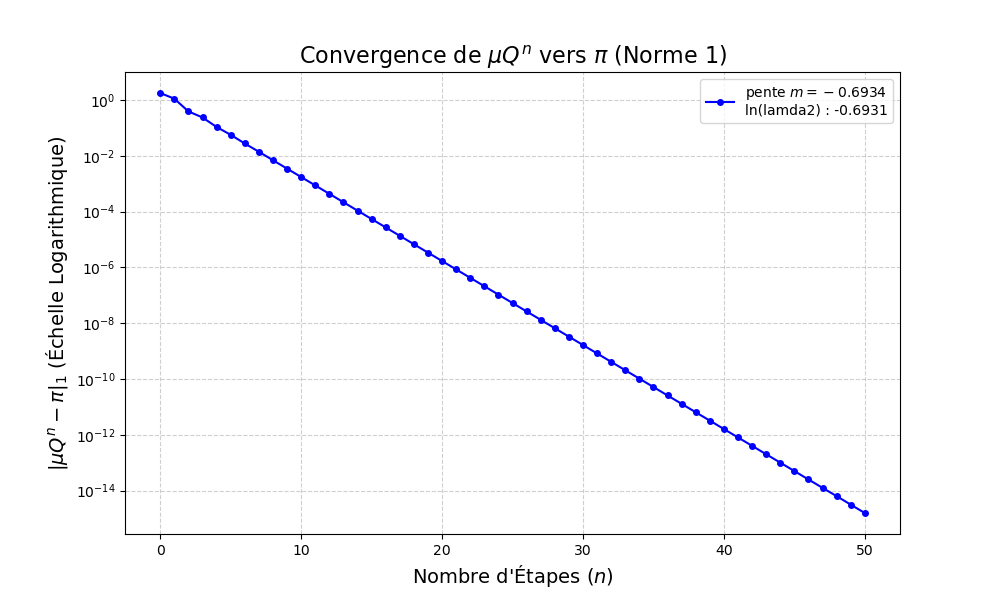
\includegraphics[width=\textwidth]{courbe_cv_exp.png}
      \\ \tiny{Décroissance exponentielle}
    \end{column}
  \end{columns}
\end{frame}


%3 Django
\begin{frame}{Dimension 2 :Périodicité et configurations en damier}
\begin{itemize}
  \item On considère l’automate de l’électeur en dimension $d=2$ avec voisinage de von Neumann (horizontal et vertical).
  \item \textbf{Grilles de taille paire} ($2k \times 2k$) :
  \begin{itemize}
    \item Existence d’un \textbf{damier parfait} (alternance $0/1$).
    \item Chaque cellule est entourée uniquement de voisins d’opinion opposée.
    \item Le système forme une \textbf{classe récurrente périodique de période 2}.
    \item Le damier se renverse à chaque itération : état alterné stable.
  \end{itemize}
  \item \textbf{Grilles de taille impaire} ($2k+1 \times 2k+1$) :
  \begin{itemize}
    \item Un damier parfait est impossible.
    \item Les motifs alternés sont instables.
    \item La chaîne converge vers un état absorbant homogène (tout $0$ ou tout $1$).
  \end{itemize}
\end{itemize}
\end{frame}

%3 Django
\begin{frame}{Influence des conditions aux bords et simulations}
\begin{itemize}
  \item \textbf{Bords fixés à 1} :
  \begin{itemize}
    \item Simulation sur une grille centrale $5 \times 5$ avec encadrement fixe de $1$.
    \item Convergence systématique vers l’état absorbant \textbf{tout-1}.
    \item Temps moyen d’absorption :
    \begin{itemize}
      \item majorité initiale de $1$ : $\bar{T} \approx 2{,}18$,
      \item majorité initiale de $0$ : $\bar{T} \approx 3{,}00$.
    \end{itemize}
    \item Les conditions aux bords imposent un biais qui domine la dynamique.
  \end{itemize}
  \item \textbf{Bords périodiques, $N=5$} :
  \begin{itemize}
    \item Temps d’absorption moyen : $\bar{T} \approx 46{,}83$ (10 000 simulations).
    \item Lorsque l’opinion est initialement dominante, le consensus correspondant apparaît dans
    $57{,}84\%$ des cas.
  \end{itemize}
\end{itemize}
\end{frame}

\section{Classes Absorbantes et Périodicité}


%-----Partie RACIM -------------------------------
\begin{frame}{Cas $N=4$ : états homogènes et états alternés}

\small

\begin{columns}

% -------- LEFT --------
\begin{column}{0.50\textwidth}

\textbf{États homogènes}

\medskip
\textbf{A :} $0000$ — tous les électeurs ont l’opinion $0$ 
\\
\textbf{B :} $1111$ — tous les électeurs ont l’opinion $1$

\medskip
Ces configurations correspondent à un \emph{consensus global}.

\medskip

\textbf{États alternés}

\medskip
\textbf{C :} $0101$ — opinions alternées entre voisins  
\\
\textbf{D :} $1010$ — même motif, décalé d’un cran

\medskip
Chaque électeur est entouré de voisins d’opinion opposée.

\medskip
{\scriptsize Les autres configurations sont \emph{transitoires} : elles évoluent vers l’un de ces motifs.}

\end{column}

% -------- RIGHT --------
\begin{column}{0.50\textwidth}
\centering

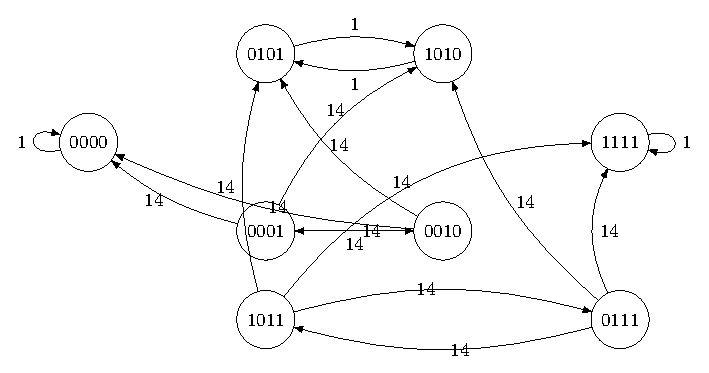
\includegraphics[width=\linewidth]{automate_N4.pdf}

\vspace{0.1cm}
{\scriptsize Automate probabiliste simplifié pour $N=4$}
\end{column}

\end{columns}

\end{frame}



\begin{frame}{Cas $N=4$ : classes absorbantes et périodicité (zoom)}

\small

% Réduction modérée de l’espace autour des formules
\setlength{\abovedisplayskip}{5pt}
\setlength{\belowdisplayskip}{5pt}

\begin{columns}

% -------- LEFT --------
\begin{column}{0.55\textwidth}

\textbf{Notation.}
\[
A=0000,\quad B=1111,\quad C=0101,\quad D=1010.
\]

\vspace{0.05cm}

\textbf{États absorbants.}
\[
P(A\to A)=1,\qquad P(B\to B)=1.
\]

\vspace{0.05cm}

\textbf{Classe récurrente \{C,D\}.}
\[
P(C\to D)=1,\qquad P(D\to C)=1.
\]

\vspace{0.05cm}

\textbf{Période (définition).}
\[
\mathcal{N}(i)=\{\,n\ge1 \mid \mathbb{P}(X_n=i \mid X_0=i)>0\,\},
\]
\[
d(i)=\mathrm{pgcd}(\mathcal{N}(i)).
\]

\vspace{0.05cm}

\textbf{Application.}
\[
\mathcal{N}(C)=\{2,4,6,\dots\}
\Rightarrow
d(C)=2 \quad(d(D)=2).
\]

\textbf{$\Rightarrow$ classe récurrente périodique de période 2.}

\end{column}

% -------- RIGHT --------
\begin{column}{0.45\textwidth}
\centering

\vspace{-0.2cm} % <-- remonte les zooms

\textbf{Zoom : états absorbants}

\vspace{0.08cm}
\begin{tikzpicture}[
  -latex,
  state/.style={circle, draw, minimum size=8mm},
  node distance=2cm
]
  \node[state] (A) {A};
  \node[state, right of=A] (B) {B};

  \path (A) edge[loop left]  node {\scriptsize $1$} (A);
  \path (B) edge[loop right] node {\scriptsize $1$} (B);
\end{tikzpicture}

\vspace{0.25cm}

\textbf{Zoom : classe \{C,D\}}

\vspace{0.08cm}
\begin{tikzpicture}[
  -latex,
  state/.style={circle, draw, minimum size=8mm}
]
  \node[state] (C) at (0,0) {C};
  \node[state] (D) at (2.6,0) {D};

  \path (C) edge[bend left=20] node[above] {\scriptsize $1$} (D);
  \path (D) edge[bend left=20] node[below] {\scriptsize $1$} (C);
\end{tikzpicture}

\vfill 
\vspace{0.15cm} 

\fbox{\parbox{0.95\linewidth}{\scriptsize
\textbf{Simulations} ($m=10^4$, $n=10^5$) :
$\mathbb{P}(A)\approx0{,}23$,
$\mathbb{P}(B)\approx0{,}31$,
$\mathbb{P}(C)\approx0{,}23$,
$\mathbb{P}(D)\approx0{,}23$.
}}

\end{column}

\end{columns}

\end{frame}

%-----fin Partie RACIM -------------------------------

\section{Dimension 2 et Influence du nombre d'opinions}

\begin{frame}{Dimension $d=2$ : Géométrie et Bords}
  \begin{itemize}
    \item \textbf{Bords fixés (1)} : Convergence systématique vers l'état "tout-1"[cite: 499].
    \item \textbf{Influence de la parité} (Bords périodiques)[cite: 489]:
    \begin{itemize}
        \item \textbf{Taille paire} : Possibilité de motifs "damier" périodiques stables[cite: 491, 504].
        \item \textbf{Taille impaire} : Convergence obligatoire vers un consensus homogène[cite: 494, 495].
    \end{itemize}
  \end{itemize}
  \end{frame}


% ----------- 2eme partie RACIM -------------------------
\begin{frame}{Influence du nombre d’opinions $\kappa$ : justification mathématique}

\footnotesize
\setlength{\abovedisplayskip}{4pt}
\setlength{\belowdisplayskip}{4pt}

\textbf{Hypothèses.}
Opinions initiales i.i.d. uniformes sur $\{0,\dots,\kappa-1\}$ ; voisinage de von Neumann (4 voisins).

\medskip
\textbf{Voisinage totalement polarisé (4--0).}
Pour une opinion fixée $c$ :
\[
\mathbb{P}(\text{4 voisins}=c)=\left(\frac{1}{\kappa}\right)^4
\quad\Rightarrow\quad
\mathbb{P}(\text{4 voisins identiques})=\kappa\left(\frac{1}{\kappa}\right)^4=\frac{1}{\kappa^3}.
\]

\medskip
\textbf{Majorité stricte (3--1 ou 4--0).}
\[
\mathbb{P}(\text{3 voisins}=c,\ 1\neq c)=\binom{4}{3}\left(\frac{1}{\kappa}\right)^3\left(\frac{\kappa-1}{\kappa}\right).
\]
En sommant sur $c$ et en ajoutant le cas 4--0 :
\[
\mathbb{P}(\text{majorité stricte})
=\kappa\binom{4}{3}\left(\frac{1}{\kappa}\right)^3\left(\frac{\kappa-1}{\kappa}\right)+\frac{1}{\kappa^3}
=\frac{4(\kappa-1)+1}{\kappa^3}=\frac{4\kappa-3}{\kappa^3}=O\!\left(\frac{1}{\kappa^2}\right).
\]

\medskip
\textbf{Conclusion.} Quand $\kappa$ augmente, les voisinages très polarisés deviennent rares $\Rightarrow$
la coalescence est ralentie et le temps d’absorption augmente.

\end{frame}

\begin{frame}{Influence de $\kappa$ : validation numérique (cas $\kappa=3$)}

\small

\textbf{Protocole}
\begin{itemize}
  \item Grille centrale $5\times 5$, voisinage de von Neumann
  \item $M=10^4$ simulations indépendantes
  \item Mesure : temps moyen d’absorption $\bar T$ + corrélation (final = majorité initiale)
\end{itemize}

\medskip

\begin{columns}
% ---- LEFT : bords libres ----
\begin{column}{0.52\textwidth}
\textbf{Bords non fixés (libres)}
\fbox{\parbox{0.95\linewidth}{\scriptsize
$\kappa=3$ : \ \ $\bar T \approx 56{,}17$ itérations.
}}

\medskip
\begin{itemize}
  \item Convergence plus lente (compétition entre opinions)
  \item Cohérent avec la raréfaction des majorités locales quand $\kappa$ augmente
\end{itemize}
\end{column}

% ---- RIGHT : bords fixés ----
\begin{column}{0.48\textwidth}
\textbf{Bords fixés (opinion imposée $b$)}
\fbox{\parbox{0.95\linewidth}{\scriptsize
$\kappa=3$ : \ \ $\bar T \approx 16{,}8$ (beaucoup plus rapide).\\
Corrélation : $b=2$ : $2871/10000$,\quad $b=0$ : $3779/10000$.
}}

\medskip
\begin{itemize}
  \item Le bord injecte en continu l’opinion $b$
  \item Biais vers $b$ : absorption accélérée
\end{itemize}
\end{column}
\end{columns}

\end{frame}

% -----------FIN  2eme partie RACIM -------------------------


\section{Conclusion}

\begin{frame}{Conclusion}
  \begin{itemize}
    \item \textbf{Finitude et Géométrie} : La taille et la parité de la grille dictent la nature des classes finales (absorbantes ou périodiques)[cite: 557].
    \item \textbf{Conditions aux bords} : Facteur dominant pour la vitesse et l'issue de la convergence[cite: 502, 556].
    \item \textbf{Fiabilité Numérique} : Les simulations corroborent systématiquement les calculs théoriques (matrices de transition, valeurs propres)[cite: 553, 557].
  \end{itemize}
\end{frame}

\end{document}